\Large
\newpage
\section*{Введение}
\addcontentsline{toc}{section}{\tocsecindent{Введение}}

Инновационный проект – это система взаимоувязанных целей и средств их достижения. Он представляет собой комплекс научно-исследовательских, опытно-конструкторских, производственных, организационных, финансовых, коммерческих и других мероприятий, соответствующим образом организованных (увязанных по ресурсам, срокам и исполнителям), оформленных комплектом проектной документации. Он должен обеспечить эффективное решение конкретной научно-технической задачи (проблемы), выраженной в количественных показателях и приводящей к инновации.

Жизненный цикл инновационного проекта, как и любой другой проектной задачи, подчиняется определенным закономерностям. В нем последовательно включены основные элементы инновационного проекта и две краеугольные временные точки: моменты запуска и закрытия. Внутренние этапы создания новшеств по своему составу зависят от вида, внутренней наполненности и масштабов проекта. Вехи как контрольные точки принятия судьбоносных решений обладают особой спецификой.

Любой проект внедряется в реально существующую внешнюю среду: на
входе проект черпает из нее ресурсы для создания продукции или оказания
каких-либо услуг, а на выходе – среда принимает результаты проектной
деятельности. Для успеха проекта нельзя не учитывать его взаимодействие с
внешней средой, что осуществляется путем комплексной экспертизы проекта –
системного, взаимосвязанного исследования внутренней и внешней среды
проекта. Всякий проект для своего осуществления нуждается в ресурсах –
финансовых, материальных, трудовых, информационных – для осуществления
как процесса производства, так и процесса управления.

Целью данной работы является планирование инновационного проекта, в
частности – магазина по продаже смартфонов. В процессе планирования можно
выделить несколько задач: кому, в какое время и какие виды работ в процессе
подготовки и реализации проекта необходимо выполнить; какие ресурсы
потребуются на выполнение каждого вида работа; определение годовой
прибыли, среднего маржинального объема реализации и порога
рентабельности.

В качестве метода управления проектами был выбран метод критического
пути, т. к. он устанавливает соотношения между затратами и длительностью
проекта, и он не учитывает случайные колебания длительности работ. Так же
проект состоит из точно определенного количества работ и для каждой работы
известна длительность выполнения. Предполагается, что длительность работы
пропорциональна объему выделяемых ресурсов, т. к. изменяя их количество,
можно изменить длительность работы и уменьшить сроки выполнения проекта.
\newpage
\section*{Выбор предприятия}
\addcontentsline{toc}{section}{\tocsecindent{Выбор предприятия}}
В качестве предприятия мною был выбран магазин смартфонов, планируется розничная продажа полностью укомплектованных смартфонов.
В качестве оказанной услуги (выпускаемой продукции) будет считаться один проданный смартфон.
\newpage
\section*{Комплекс работ}
\addcontentsline{toc}{section}{\tocsecindent{Комплекс работ}}

Определим комплекс работ (событий), подлежащих выполнению и продолжительность выполнения работ. Сформулируем содержание работ (событий) и представим перечень событий и работ в таблице 1.

\begin{table}[h!]
	\caption{Комплекс работ}
	\begin{tabular}{|p{1cm}|p{9cm}|p{3cm}|p{3cm}|}
	\hline
	Номер события & Событие & Предыдущее событие & Продолжительность события, неделя \\
	\hline
	1 & Регистрация юридического
	лица и регистрация в
	налоговых службах
 & - & 2 \\
	\hline
	2 & Поиск помещения & 1 & 3 \\
	\hline
	3 & Аренда помещения & 2 & 1 \\
	\hline
	4 & Ремонт помещения & 3 & 8 \\
	\hline
	5 & Поиск поставщика & 1 & 1 \\
	\hline
	6 & Закупка и поставка смартфонов & 5 & 2 \\
	\hline
	7 & Проверка оборудования на дефекты & 6 & 1 \\
	\hline
	8 & Поиск и найм персонала & 6 & 2 \\
	\hline
	9 & Обучение персонала & 8 & 4 \\
	\hline
	10 & Запуск рекламной компании & 6 & 3 \\
	\hline
	11 & Cоздание интернет инфраструктуры (сайт, база данных и т.д.) & 10 & 2 \\
	\hline

\end{tabular}
\end{table}
\newpage
\section*{Сетевой график выполнения комплекса работ}
\addcontentsline{toc}{section}{\tocsecindent{Сетевой график выполнения комплекса работ}}

Теперь построим сетевой график выполнения комплекса работ (событий), а также определим критический путь и его продолжительность.

Сетевой график представлен на рисунке 1. 

\begin{figure}[h!]
	\caption{Сетевой график выполнения комплекса работ}
\center{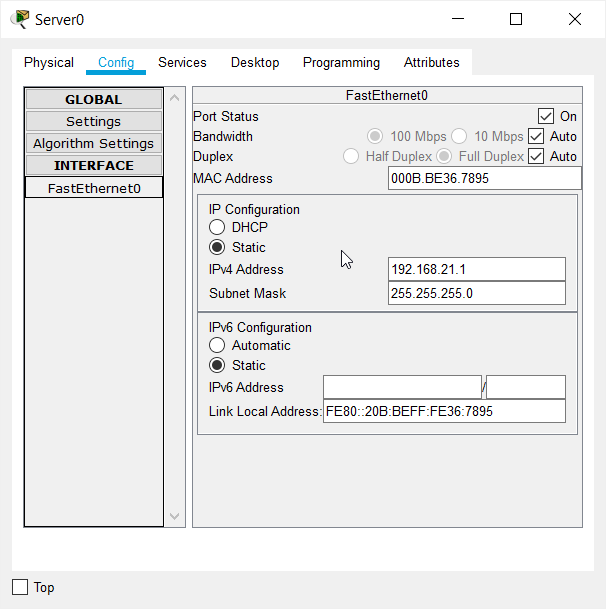
\includegraphics[scale=0.4]{1}}
\end{figure}

Критический путь — самый продолжительный путь сетевого графа (состоит из
событий с нулевым резервом времени).

Критический путь: 1 → 2 → 3 → 4 → 10

Продолжительность критического пути — 14 недель.

\newpage
\section*{Перечень переменных и постоянных затрат}
\addcontentsline{toc}{section}{\tocsecindent{Перечень переменных и постоянных затрат}}

Определим номенклатуру переменных и постоянных затрат.

Постоянные затраты — затраты, величина которых в краткосрочном периоде
(не меняется производственная мощность) не меняется при изменение объемов
выпускаемой продукции. Примеры: затраты на аренду и оборудование,
амортизация, проценты по кредитам и ЗП управленческому, вспомогательному
персоналу и др.

В таблице 2 представлены постоянные затраты текущего проекта.
\begin{table}[h!]
	\caption{Постоянные затраты текущего проекта}
\begin{tabular}{|p{12cm}|p{4cm}|}
	\hline
	Услуга & Цена, руб. \\
	\hline
	Аренда помещения & 50 000 \\
	\hline
	Заработная плата управленческому и
	вспомогательному персоналу
 & 150 000 \\
	\hline
	Реклама магазина & 25 000 \\
	\hline
	Подоходный налог (основной вид прямых
	налогов, исчисляется в процентах от
	совокупного дохода физических или
	юридических лиц за вычетом документально
	подтвержденных расходов, в соответствии с
	действующим законодательством) & 30 000 \\
	\hline
	Запас оборотных средств & 500 000 \\
	\hline
	Отчисления в ПФР (в размере 22\% от фонда
	оплаты труда работника) & 55 000 \\
	\hline
	Прочие расходы & 20 000 \\
	\hline
\end{tabular}
\end{table}

Итого постоянных затрат (за год): 830 000 * 12 = 9 960 000 руб.

Переменные затраты — затраты, величина которых меняется при изменении
объемов выпускаемой продукции. Примеры: затраты на покупку сырья,
материалов, ЗП рабочих, топливо, энергия и др.

В таблице 3 представлены переменные затраты текущего проекта.

\begin{table}[h!]
	\caption{Переменные затраты текущего проекта}
	\begin{tabular}{|p{12cm}|p{4cm}|}
		\hline
		Услуга & Цена, руб. \\
		\hline
		Покупка телефонов & 1 000 000 \\
		\hline
		Заработная плата рабочим
 & 75 000 \\
		\hline
		Гигиенические принадлежности и расходные материалы & 20 000 \\
		\hline
		Коммунальные платежи & 15 000 \\
		\hline
	\end{tabular}
\end{table}

Итого переменных затрат (за год): 1 110 000 * 12 = 13 320 000 руб.

Теперь получим общие затраты в месяц и год:

Общие затраты в месяц - 1 940 000 руб.

Общие затраты в год - 23 280 000 руб.

\newpage
\section*{Средняя цена реализации единицы продукции}
\addcontentsline{toc}{section}{\tocsecindent{Средняя цена реализации единицы продукции}}

Определим среднюю цену реализации (руб.) единицы продукции (услуги).

Цена реализации - это та цена, по которой продают продукцию. Она напрямую зависит от многих факторов: состояния рынка, средних цен на аналогичные предложения, себестоимости и затрат на производство, наличия конкурентов и т.п. 

Для определения средней цены чаще всего используют формулы расчета величин: средней арифметической, средней арифметической взвешенной и средней гармонической. Самый распространенный вид средней цены - значение, полученное расчетом средней арифметической величины. Ее применяют тогда, когда необходимо вычислить среднее слагаемое в общей совокупности данных.

Для того, чтобы вычислить среднюю цену, необходимо воспользоваться
формулой (1) для подсчета с помощью среднеарифметической цены:

\begin{align}
\text{СредЦена} = \frac{\text{СУММА} (P_i \cdot V_i)}{\text{СУММА}(V_i)},
\end{align} где $P_i$ – цена товара за период реализации; $V_i$ – объем товара, по которому
считается средняя цена за все периоды реализации.

Имеем:
\begin{enumerate}
	\item В первое полугодие: 450 смартфонов по цене 25 000 руб. за штуку.
	\item Во втором полугодии: 300 смартфонов по цене 33 000 руб. за штуку.
\end{enumerate}

Откуда получим, что

\begin{align}
\text{СредЦена} = \frac{450 \cdot 25 000+300 \cdot 33 000}{750} = 28 200 \text{руб}.
\end{align}

Средняя цена товара - 28 200 руб.

\newpage
\section*{Планируемый объем производства}
\addcontentsline{toc}{section}{\tocsecindent{Планируемый объем производства}}

Планирование объема производства продукции представляет собой процесс
сбора данных о предполагаемом выпуске готовых изделий в единую
программу, в стоимостном и натуральном измерениях. Планирование
производства и сбыта продукции относится к управленческой деятельности
предприятия. Планируемый объем производства продукции определяют на
основании договором с заказчиками и собственных потребностей, а также с
учетом стратегического развития предприятия. Если предприятие находится на
начальной стадии развития, обязательно разрабатывают прогноз выпуска
продукции, базирующийся на маркетинговых исследованиях.

Установим планируемый объем производства продукции (работы, услуги) в год.

Прогноз выпуска продукции:
\begin{enumerate}
	\item В первом квартале планируется выпускать 150 шт.
\item  Во втором квартале планируется выпускать 350 шт.
\item Во третьем квартале планируется выпускать 280 шт.
\item Во четвертом квартале планируется выпускать 220 шт.
\end{enumerate}

Следовательно, планируемый объем производства продукции в год - 1 000 штук.

\newpage
\section*{Годовая прибыль}
\addcontentsline{toc}{section}{\tocsecindent{Годовая прибыль}}

Чистой прибылью считаются денежные средства, оставшиеся у компании после
того, как из балансовой выплатили все налоги, взносы и другие обязательные
платежи. Чистая прибыль остается в компании и является финансовым
источником, идущим на различные нужды фирмы, развитие производственной
базы, формирование резервных и поощрительных фондов, увеличение
оборотного капитала, выплату дивидендов.

На образование чистой прибыли оказывают влияние:
\begin{enumerate}
	 \item доходы от продажи товаров или выполнения услуг;
\item себестоимость произведенной продукции;
\item размеры обязательных платежей, в т.ч. налоговых.
\end{enumerate}

Расчет прибыли – это определение разницы между объемом полученной
выручки и затратами. Годовая прибыль вычисляется по формуле 4:
\begin{align}\text{Годовая Прибыль}=\text{Выручка}-\text{Общие затраты} \end{align}

Следовательно, в нашем случае получим, что 
\begin{align}\text{ГодПрибыль} = 1 000 \cdot 28 200 - 23 280 000 = 4 920 000 \text{руб}.
\end{align}

Годовая Прибыль - 4 920 000 руб.

\newpage
\section*{Маржинальный доход}
\addcontentsline{toc}{section}{\tocsecindent{Маржинальный доход}}

Маржинальный доход - разница между выручкой предприятия от реализации продукции (работ, услуг) и суммой переменных затрат. 

Маржинальный доход вычисляется по формуле 5:
\begin{align}\text{Маржинальный Доход}=\text{Выручка}-\text{Переменные затраты} \end{align}

Получим, что 
\begin{align}\text{МаржДоход} = 1 000 \cdot 28 200 - 13 320 000 = 14880000 \text {руб.}
\end{align}

Под средней величиной маржинального дохода понимают разницу между средней ценой продукции и средними переменными затратами. Средняя величина маржинального дохода отражает вклад единицы продукции в покрытие постоянных затрат и получение прибыли.

Средняя величина маржинального дохода вычисляется по формуле 7:
\begin{align}\text{Средняя Величина Маржинального Дохода}=\frac{\text{Маржинальный доход}}{\text{Объем реализации}} \end{align}

Откуда получим, что 
\begin{align}\text{СредМаржДоход} = \frac{14880000}{1000} = 14880 \text {руб.}
\end{align}

Средняя величина маржинального дохода - 14 880	 $\frac{\text{руб.}}{\text{шт.}}$.

\newpage
\section*{Порог рентабельности}
\addcontentsline{toc}{section}{\tocsecindent{Порог рентабельности}}

Найдем порог рентабельности (точку безубыточности).

Точка безубыточности — это такое значение объема продаж, при котором
совокупные затраты равны совокупной выручке, то есть предприятие не
получает ни прибыли, ни убытков.
Для того, чтобы вычислить точку безубыточности, необходимо использовать
формулу 9.
\begin{align}\text{ТБ}=\frac{\text{Постоянные затраты}}{\text{Цена реализации ед. прод.}- \text{Переменные затраты на ед. прод.}} \end{align}

Следовательно, используя формулу 9, получим:
\begin{align}\text{ТБ}=\frac{
9 960 000}{28200 - \frac{13 320 000}{1000}} =670\text{шт.
}
\end{align}
Точка безубыточности - 670 шт.

\newpage
\section*{Прибыль предприятия}
\addcontentsline{toc}{section}{\tocsecindent{Прибыль предприятия}}

Таким образом, вся информация о прибыли предприятия при установленном объеме реализации продукции представлена в таблице 4.

\begin{table}[h!]
	\caption{Прибыль предприятия при установленном объеме реализации продукции (работ, услуг)}
	\begin{tabular}{|p{1cm}|p{8cm}|p{7cm}|}
		\hline
		№ & Показатель & Значение \\
		\hline
		1 & Объем производства  & 1 000 шт. \\
		\hline
		2 & Выручка от реализации & 28 200 000 руб. \\
		\hline
		3 & Переменные затраты  & 13 320 000 руб. \\
		\hline
		4 & Маржинальный доход & 14 880 000 руб. \\
		\hline
		5 & Постоянные затраты & 9 960 000 руб. \\
		\hline
		6 & Годовая прибыль & 4 920 000 руб.  \\
		\hline
		7 & Средняя величина маржинального дохода & 14  880$\frac{\text{руб.}}{\text{шт.}}$ \\
		\hline
	\end{tabular}
\end{table}
\newpage
\section*{Заключение}
\addcontentsline{toc}{section}{\tocsecindent{Заключение}}
Таким образом, в результате выполнения данного домашнего задания
\begin{enumerate}
	 \itemбыли получены теоретические знания о том, как  правильно спланировать
	инновационный проект;\item были приобретены навыки расчета выручки продукции, валовой маржи,
	средней цены изделия, точки безубыточности, а также расчета
	издержек;\item и, наконец, был спланирован инновационный проект.
\end{enumerate}
